\documentclass[compress,dvips,xcolor={dvipsnames},t]{beamer}

\usepackage[english]{babel}
\usepackage{graphicx}
\usepackage{amssymb,amsmath}
%\usepackage{url}
\usepackage{xspace}
\usepackage{hyperref}

\renewcommand{\refname}{}
\newcommand\ASN{\textsf{ASN.1}\xspace}
\newcommand\Cpp{\mbox{\textsf{C} \hspace*{-2.5mm} \raise 0.7mm \hbox 
{${\scriptscriptstyle \textsf{++}}$}}\xspace}

\newcounter{savedenum}
\newcommand*{\saveenum}{\setcounter{savedenum}{\theenumi}}
\newcommand*{\resume}{\setcounter{enumi}{\thesavedenum}}

\title{Case study: compiling \ASN}
\author{Christian Rinderknecht}
\date{27 February 2013}

\begin{document}

\frame{\maketitle}

\begin{frame}
\frametitle{Statement of Purpose}

The purpose of this presentation is to convince you that I can handle
a \Cpp frontend and use it to implement whatever static analysis I
design that is needed by the embedding application.

\bigskip

Whilst I used to program in \Cpp quite often ten years ago, I have
since become a casual \Cpp programmer, as this is not a suitable
language for writing compilers, if given the choice (especially
frontends).

\bigskip

I do not expect this confession to be a serious impediment, though, as
I always master a comprehensible subset of each programming language I
use, and I fancy myself as a sort of linguist.

\end{frame}

%%%%%%%%%%%%%%%%%%%

\begin{frame}
\frametitle{What this could have been about}

In 2008 and 2010, Nic Volanschi (Metaware) and I published papers
about a new technique we call \emph{unparsed patterns}, and how to use
them to extend an existing compiler (here, GCC \Cpp) with user-defined
checks. For full details, please read the following:
\begin{itemize}

  \item conference version: {\small\url{http://home.konkuk.ac.kr/~rinderkn/pub/pepm2008.pdf}}

  \item journal version (extended): {\small\url{http://home.konkuk.ac.kr/~rinderkn/pub/scp2010.pdf}}

\end{itemize}
The reason why I won't be presenting this is that it is a joint work:
Nic had the original idea and implemented it on GCC. I contributed by
simplifying the algorithms, expressing them in formal logic (also
OCaml and Prolog), and proving desirable properties about them.

\medskip

Of course, this work has everything to do with compilers, but the
approach to frontends is unusual: the core idea is to avoid modifying
them as much as possible and not parsing at all.

\end{frame}

%%%%%%%%%%%%%%%%%%%

\begin{frame}
\frametitle{What this is about}

Instead, I will present a past project, which started long time ago,
during my Ph.D., and which has become my pet project along these
years: compiling \ASN.

\bigskip

This language is a good case study for a frontend, because it is
extremely hard to parse and analyse.

\bigskip

Also, code generation requires a good knowledge of low-level wizardry,
down to packing the bits in the frames.

\end{frame}

%%%%%%%%%%%%%%%%%%%

\begin{frame}
\frametitle{\ASN}

\emph{Abstract Syntax Notation One} (\ASN) is a standardised language
(ISO, ITU-T) for defining data types whose values may be exchanged
across a network between two, possibly heterogeneous peers. It is used
in the following contexts.

\begin{itemize}

  \item Telecommunication Management Network (SNMP, CMIP);

  \item Lightweight Directory Access Protocol (LDAP);

  \item email (\textsf{X.400});

  \item \textsf{UMTS} (Radio Access Network);

  \item Transferred Account Procedure~3 (billing for
    \textsf{GSM/UMTS} roaming);

  \item \textsf{3GPP LTE} (Long Term Evolution of \textsf{GSM/UMTS}
    networks);

  \item Multimedia conferencing systems with \textsf{H.323} (for
    signalling: \textsf{H.225}, \textsf{H.235}, \textsf{H.245},
    \textsf{H.248}, \textsf{H.450.1});

  \item Interactive television services (\textsf{MHEG});

\end{itemize}

\end{frame}

%%%%%%%%%%%%%%%%%%%

\begin{frame}
\frametitle{\ASN (usages, continued)}

\begin{itemize}

  \item Intelligent Transportation Systems (traffic signal
  control, electronic toll collection, emergency response etc.);

  \item Radio Frequency Identification (RFID);

  \item Aeronautical Telecommunication Network (air traffic control,
    flight information services, passenger communications, air-ground
    protocols etc.);

  \item Cryptography for electronic commerce over the internet (SET,
    PKCS~7, OpenSSL);

  \item Smart cards (SIM, WIM and VITALE);

  \item National Center for Biotechnology Information (NCBI):
    specification of millions of DNA sequences;

  \item client-server protocol for database access (U.S. Library of
    Congress: \textsf{Z39.50});

  \item \emph{and many more.}

\end{itemize}

\end{frame}

%%%%%%%%%%%%%%%%%%%

\begin{frame}
\frametitle{Why \ASN?}

\begin{itemize}

\item It is an abstract language for expressing types and network
  concepts, independently of any programming language. As a
  specification language, it is embedded in other languages,
  \emph{e.g.}, \textsf{SDL} (modelling of protocols with extended
  finite state machines) and \textsf{MSC} (functional requirements
  with interaction scenarios), \textsf{TTCN} (test suites) etc.

 \item Beyond types, it features network concepts.

\item When used to implement telecommunication protocols, it comes
  associated with \emph{encoding rules}, which specify how to
  serialise an \ASN value.

  \item These encoding rules, like the Packed Encoding Rules
  (\textsf{PER}) are specially optimised for \ASN in order to save
  bandwith (although they can be tuned for saving codec time).

\end{itemize}

\end{frame}

% \item Culture wars: first, \ASN was not born in the internet world,
%   and, now, it is not \textsf{XML}.

\begin{frame}
\frametitle{\ASN and the compilation chain}

\begin{center}
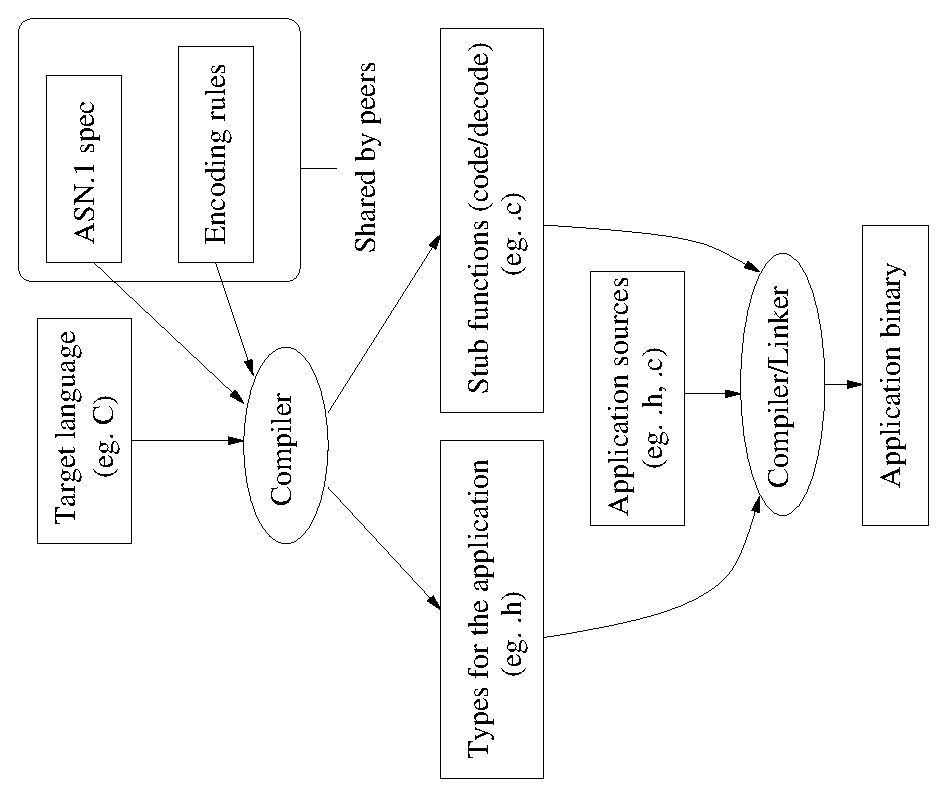
\includegraphics[scale=0.5]{compilation.eps}
\end{center}

\end{frame}

%%%%%%%%%%%%%%%%%%%

\begin{frame}
\frametitle{\ASN/BER and telecommunication}

\begin{center}
\includegraphics[scale=0.45]{model-1.eps}
\end{center}

\end{frame}

\begin{frame}
\frametitle{Issues}

\begin{enumerate}

  \item Specifications: huge (704 pages A4 10pt), complex (concepts
  mutually dependent).

  \item Syntax: large and ambiguous grammar, dynamic extensions.

  \item English cannot tell the meaning of all combinations of
    syntactical constructs.
  
  \item Types denote value sets and type operators denote set
    operations: subtypes yield general set constraints.

  \item Encoding only applies to a subset of \ASN, defined
    implicitly and dependent on the encoding rules.

  \item Decoding is unspecified.

  \item Dynamic checks in codecs (depending on the target programming
    language) are unspecified.

  \item Open source or free compilers: extremely rare, unmaintaned,
    fragile, without precise error reporting.

\end{enumerate}

\end{frame}

%%%%%%%%%%%%%%%%%%%

\begin{frame}
\frametitle{Syntax analysis}

The BNF of \ASN spans 23~pages, versus 19~pages for ISO \Cpp.

\bigskip

When fed to Yacc as it is specified in the standards, it yields
between 3,000 and 4,000 shift/reduce and reduce/reduce conflicts
(for each kind!). It is ambiguous too.

\bigskip

The situation is actually much worse: many \emph{tokens} are
ambiguous, so if the lexer works without any extra knowledge from the
parser, there are even more conflicts.

\bigskip

I first solved the problem of the syntax analysis on the 1990
standard, which is smaller, albeit very nasty as well.

\end{frame}

%%%%%%%%%%%%%%%%%%%

\begin{frame}
\frametitle{Syntax analysis of \ASN 1990}

Too often engineers expect an off-the-shelf tool that will solve
parsing problems. If Yacc is put to work, 
\begin{itemize}

\item it may not be suited for precise error reporting (bottom-up
  parsing, whilst more powerful than top-down, is really bad at
  providing syntactical context)

\item and understanding conflicts is done on the automaton, hence
  obscuring the relationship between the conflicts and the grammar
  (the parsing algorithm must be clearly held in mind at all times,
  because a conflict may involve several productions and a
  modification in one of them will change the automaton).

\end{itemize}

\bigskip

Real ingenuity and fortitude is needed, and I met an engineer who quit
after working six months on the syntax of \ASN (the company gave up
and is still paying an expensive license for a frontend).

\end{frame}

%%%%%%%%%%%%%%%%%%%

\begin{frame}
\frametitle{Syntax analysis of \ASN 1990 (cont.)}

Nevertheless, I devised a method and tools that help. It took me three
months to obtain an LL(1) grammar of \ASN and the corresponding
recursive descent parser, which was mathematically proved correct and
complete with respect to the standard BNF, and which reported syntax
errors very accurately. See
\begin{itemize}

  \item in French: 
{\small\url{http://home.konkuk.ac.kr/~rinderkn/pub/RT171.pdf}}

  \item in English (shorter):
{\small\url{http://konkuk.ac.kr/~rinderkn/pub/TR171-eng.pdf}}

\end{itemize}
Beyond the academic world, it was employed by some private
companies. The case I know best is that of the (ex) Southwestern Bell,
where they wanted to check the validity of their U.S. \ASN database,
used by all the subsidiaries of the group to define their
telecommunication protocols.

\end{frame}

%%%%%%%%%%%%%%%%%%%

\begin{frame}
\frametitle{Syntax analysis of \ASN 1990 (cont.)}

The programming language used to implement the parser was OCaml, but
the open source project Cryptix used the underlying, LL(1) grammar to
reimplement my parser in Java. See

\medskip

{\small\url{http://cryptix-asn1.sourceforge.net/ASN1-004.grammar}}

\medskip

Cryptix is an early library (still in use) for programming
cryptography in Java. (Check the ChangeLog file and search for errors
related to ``parsing''.)

\end{frame}

%%%%%%%%%%%%%%%%%%%

\begin{frame}
\frametitle{Syntax analysis of \ASN 2008?}

I have been working on the latest \ASN standards and the current
grammar. The increase in size and complexity are still amenable to the
same method as the 1990 version, but a summary of the transformations
to reach the form LR(1) spans more than 60~pages (versus~45 for the
1990 version). And it is not even LL(1)!

\bigskip

To alleviate the problem, I am writing a tool to check the grammar
transformations, which are algebraic in nature because we are dealing
with a context-free language. Moreover, if OCaml is used for the
semantic actions, I can automatically construct the abstract syntax
trees for the final grammar (mapping the algebraic transformation on
the concrete syntax onto the abstract syntax).

\bigskip

Nevertheless, future changes to the grammar probably would invalidate
an unpredictable amount of previous work, so I have been investigating
another approach as well.

\end{frame}

%%%%%%%%%%%%%%%%%%%

\begin{frame}
\frametitle{Another approach}

The technique I am envisaging now consists in extending the tool used
to perform and check the transformations by adding the possibility of
\emph{stratifying} the grammar.

\bigskip

This means that we can separate different syntactic layers to reduce
parsing conflicts and isolate potential changes. 

\bigskip

Moreover, we can type top-level identifiers from the layer of
definitions and feed them the lexer \emph{again} (feedback from the
parser) so we parse the file multiple times, each time with more
typing information and focusing on different parts of the grammar.

\bigskip

But let us move to the static analysis of \ASN.

\end{frame}

%%%%%%%%%%%%%%%%%%%

\begin{frame}[containsverbatim]
\frametitle{Examples of problems}

\begin{itemize}

  \item An incorrect specification is rejected too late:\\
        \verb+T ::= T+ \ \ yields \ \ \verb+typedef T T;+\\
        which is rejected by the C compiler.

\bigskip

  \item A correct specification is rejected:
\begin{verbatim}
T ::= SET (WITH COMPONENT (0) 
          | WITH COMPONENT (1)) OF INTEGER
\end{verbatim}

\bigskip

   \item An incorrect specification is accepted:\\
         \verb+a INTEGER (0<..9) ::= 0+

\end{itemize}

\end{frame}

%%%%%%%%%%%%%%%%%%%

\begin{frame}
\frametitle{Issues in validation}

\ASN types are considered as sets of values, thus types must have at
least one (finite) value.

\bigskip

Because of the great expressivity of \ASN, the compilers are not
likely to fully check arbitrary combinations of subtyping
constraints.

\bigskip

\begin{itemize}

\item Vendors' argument: ``This is hardly a real problem because those
  critical specifications are rarely found in practice.''

\bigskip

\item My argument: ``Maintenance costs are always wildly
  underestimated. Why not solve completely the problem, get a better
  product and save money and time?''

\end{itemize}

\end{frame}


\begin{frame}
\frametitle{Problems}

\begin{enumerate}
  
  \item \label{finiteness} the types may have only infinite
        values:\\
        \texttt{T ::= SET \{a T\}}\\
        \(\rightarrow\) \emph{this is the finiteness problem;}

  \item \label{type_conformance} some value declarations may be
        ill-typed:\\
        \texttt{v REAL ::= ""}\\
        \(\rightarrow\) \emph{this is the typechecking problem;}

  \item \label{type_compatibility} especially, some value references
        may be ill-typed, as\\
        \texttt{a VisibleString ::= b}\\
        \texttt{b INTEGER ::= 0}\\
        \(\rightarrow\) \emph{this is the type compatibility problem;}

\saveenum

\end{enumerate}

\end{frame}

\begin{frame}
\frametitle{Problems (cont.)}

\begin{enumerate}

\resume

  \item \label{constraint_consistence} the subtype constraints may
        be inconsistent:\\
        \texttt{T ::= REAL (SIZE(7))}\\
        \(\rightarrow\) \emph{this is the consistence problem;}

  \item \label{subtype_non_emptyness} the subtypes may be empty, as\\
        \texttt{T ::= SET ((SIZE (1)) \symbol{94} (SIZE (2))) OF REAL}\\
        \(\rightarrow\) \emph{this is the emptiness problem;}
   
  \item \label{solvability} the subtypes may have no value set:\\
        \texttt{T ::= REAL (ALL EXCEPT T)}\\
        \(\rightarrow\) \emph{this is the solvability problem.}

\end{enumerate}

\end{frame}

\begin{frame}
\frametitle{Analysis}

\begin{itemize}

  \item type compatibility $\subseteq$ typechecking;

  \item constraint consistence, emptiness $\subseteq$ solvability
        (the system is solved when we construct explicitly the values
        of each subtype);

  \item typechecking $\subseteq$ solvability:
\begin{tabular}{@{}r@{\;}c@{\;}l@{}}
   \texttt{y INTEGER (0..9) ::= 1}
   & $\rightarrow$ 
   & $\left\{
       \begin{tabular}{l} 
           \texttt{y A ::= 1} \\
           \texttt{A ::= INTEGER (0..9)} \\
           \texttt{B ::= A (y)}
        \end{tabular}
     \right.$
\end{tabular}
where \texttt{A}~and~\texttt{B} are fresh type references.

\end{itemize}

So, finiteness and solvability are enough to get a full validation.

\end{frame}

%%%%%%%%%%%%%%%%%%%

\begin{frame}
\frametitle{Two approaches for the frontend}

Every \ASN specification is rewritten in a subset of same
expressiveness, with less syntactical constructs. Two strategies:

\begin{enumerate}

  \item Few preliminary rewrites, followed by a collection of set
  constraints, then fed to a generic constraint solver.\\
{\small\url{http://home.konkuk.ac.kr/~rinderkn/pub/cj2003.pdf}}

\bigskip

  \item Lots of preliminary rewrites, simple algorithms to check
    solvability. (This is like taking the previous method and
    interleave a dedicated solver with the syntactical rewrites.)\\
{\small\url{http://home.konkuk.ac.kr/~rinderkn/pub/these.pdf}}

\end{enumerate}

\end{frame}

%%%%%%%%%%%%%%%%%%%

\begin{frame}
\frametitle{Comparison}

\begin{enumerate}

\item Pros: modularity, less programming. Cons: constraints too
  general for off-the-shelf solvers, and translation of constraints
  needed anyway.

\item Pros: easy checking. Cons: eavily specialised, correctness hard
  to assess.

\end{enumerate}
I need to find a trade-off now.

\end{frame}

%%%%%%%%%%%%%%%%%%%

\begin{frame}
\frametitle{The Encoding Rules}

The encoding rules also need attention, both in their design and how
they are implemented by the code generators or by hand.

\bigskip

They have been frequently associated with reports of vulnerability.

\bigskip

I showed that these reports were inaccurate insofar as they pointed
the finger at the encoding rules, rather than poor implementations
produced by backends of \ASN compilers. See

\medskip

{\small\url{http://home.konkuk.ac.kr/~rinderkn/pub/sam2004.pdf}}

\end{frame}

%%%%%%%%%%%%%%%%%%%

\begin{frame}
\frametitle{Core \ASN and soundness property}

\centerline{\includegraphics[width=.85 \textwidth]{model-2.eps}}

\end{frame}


\begin{frame}[containsverbatim]
\frametitle{Short presentation of \ASN}

\noindent
\textbf{Some basic types}
\begin{itemize}

  \item \verb+ok BOOLEAN ::= TRUE+

%%  \item The \texttt{NULL} type has only one value, also noted
%%        \texttt{NULL};

  \item 

\begin{verbatim} 
zero INTEGER ::= 0 
DayInTheYear ::= INTEGER {first(1), last(356)}
newYearsEve DayInTheYear ::= last
\end{verbatim}

  \item 
\begin{verbatim}
SynchroIndicator ::= ENUMERATED {serial,parallel}
synchro SynchroIndicator ::= serial
\end{verbatim}

  \item

\begin{verbatim}
pi REAL ::= 3.14159
micron REAL ::= {mantissa 1,base 10,exponent -6}
\end{verbatim}

  \item 

\begin{verbatim}
byte BIT STRING ::= 'OD'H  -- or '00001110'B
T ::= BIT STRING {msb(7), lsb(0)}
v T ::= {msb, lsb}  -- or '10000001'B
\end{verbatim}

%%  \item The \texttt{OCTET STRING} type is similar to the \texttt{BIT
%%        STRING} for eight-bit multiples strings.

%%  \item The \texttt{OBJECT IDENTIFIER} and \texttt{RELATIVE-OID} types
%%        aim at referencing other \ASN modules (a set of type
%%        and value declarations) at an international level, by means of
%%        a path in a standard tree.

  \item For historical reasons, there are many string types.

\end{itemize}

\end{frame}

\begin{frame}[containsverbatim]
\frametitle{Some constructed types}

The \texttt{SET} type corresponds to the record-like structures in
programming languages:
\begin{verbatim}
PersonInfo ::= SET {age INTEGER, married BOOLEAN}
i PersonInfo ::= {married TRUE, age 42}
\end{verbatim}
Some fields can be marked as optional or having a default value:
\begin{verbatim}
Point ::= SET {x REAL DEFAULT 0, y REAL DEFAULT 0}
origin Point ::= {}           -- or {x 0.0, y 0.0}
\end{verbatim}

\end{frame}

\begin{frame}[containsverbatim]
\frametitle{Some constructed types (cont.)}

An excerpt from a real protocol:
\begin{verbatim}
DataAcknowledgementTPDU ::= SET {
  destRef        Reference,
  yr-tu-nr       TPDUnumber,
  checkSum       CheckSum OPTIONAL,
  subSeqNr       SubSequenceNumber DEFAULT 0,
  flowControlCnf FlowControlConfirmation OPTIONAL}
\end{verbatim}

The \texttt{SET OF} type corresponds to the mathematical notion of
sets with repetition:
\begin{verbatim}
T ::= SET OF INTEGER
empty T ::= {}
small T ::= {7, 9, 1, 1, 3}
\end{verbatim}

\end{frame}

\begin{frame}[containsverbatim]
\frametitle{Some constructed types (cont.)}

The \texttt{CHOICE} type corresponds to a \textbf{union} in C.
\begin{verbatim}
T ::= CHOICE {x REAL, y BOOLEAN}
u T ::= x : 0.5
v T ::= y : FALSE
\end{verbatim}
The Protocol Data Units (PDU) are \texttt{CHOICE} types, because they
model all the possible queries and responses between two peers. A
\texttt{CHOICE} type may be recursive, like the other constructed
types. One real example (a Network Management Protocol) is:
\begin{verbatim}
CMISFilter ::= CHOICE {
  item  FilterItem,
  and   SET OF CMISFilter,
  or    SET OF CMISFilter,
  not   CMISFilter}
\end{verbatim}

\end{frame}

\begin{frame}[containsverbatim]
\frametitle{Some subtyping constraints}

\ASN offers a very involved subtyping paradigm consisting of
constraints upon recursive types, that restricts their corresponding
sets of values in a set-theoritic manner, but also in a structural
way.
\begin{itemize}

  \item \textbf{Interval Constraint}: the \texttt{INTEGER},
  \texttt{REAL} and (almost all) string types have totally ordered
  values, hence allowing interval definitions. For instance:

\begin{verbatim}
PositiveOrZeroInteger ::= INTEGER (0..MAX)
PositiveInteger ::= INTEGER (0<..MAX)
NegativeOrZeroInteger ::= INTEGER (MIN..0)
NegativeInteger ::= INTEGER (MIN..<0)
PositiveReal ::= REAL (0<..PLUS-INFINITY)
NegativeReal ::= REAL (MINUS-INFINITY..<0)
RealInterval ::= REAL (4e-5..1e-4)
\end{verbatim}
\end{itemize}

\end{frame}

\begin{frame}[containsverbatim]
\frametitle{Some subtyping constraints (cont.)}

\begin{itemize}

  \item \textbf{Value Constraint}: to restrict the set of values of a
  type to be a singleton:

\begin{verbatim}
Wednesday ::= Day (wednesday)
\end{verbatim}

  \item \textbf{Union Constraint}: the new subtype contains the values
  of the first subtype and of the second subtype (keyword
  \texttt{UNION} or symbol \texttt{|}):

\begin{verbatim}
Day ::= ENUMERATED {monday, tuesday, wednesday, 
              thursday, friday, saturday, sunday}
WeekEnd ::= Day (saturday | sunday)
\end{verbatim}

  \item \textbf{Alphabet Constraint}: the strings can be restricted to
  be built upon a given alphabet:

\begin{verbatim}
CapitalAndSmall ::= 
  IA5String (FROM ("A".."Z" | "a".."z"))
CapitalOrSmall ::= 
  IA5STring (FROM ("A".."Z") | FROM ("a".."z"))
\end{verbatim}

\end{itemize}

\end{frame}

\begin{frame}[containsverbatim]
\frametitle{Some subtyping constraints (cont.)}

\begin{itemize}

  \item \textbf{Size Constraint}: the values of string types may be
        constrained to a given sizes, introducing a constraint by the
        keyword \texttt{SIZE}:

\begin{verbatim}
Exactly31BitsString ::= BIT STRING (SIZE (31))
StringOf31BitsAtTheMost ::=
  BIT STRING (SIZE (0..31))
NonEmptyString ::= BIT STRING (SIZE (1..MAX))
\end{verbatim}

The size constraint can also apply to \texttt{SET OF} types. In that
case, the semantics is very different: the values of the types are
sets whose \emph{cardinals} are specified by the size constraint:

\begin{verbatim}
SetOf5Strings ::=
  SET (SIZE(5)) OF PrintableString
SetOfStringsOf5Char::=
  SET OF PrintableString (SIZE(5))
\end{verbatim}

\end{itemize}

\end{frame}

\begin{frame}[containsverbatim]
\frametitle{Some subtyping constraints (cont.)}

\begin{itemize}

  \item \textbf{Intersection Constraint}: the new subtype contains the
        values that belong to the two subtypes (keyword
        \texttt{INTERSECTION} or symbol \texttt{\symbol{94}}):

\begin{verbatim}
FrenchPhoneNumber ::= 
  NumericString (FROM ("0".."9") ^ SIZE (10))
\end{verbatim}

  \item \textbf{Inclusion Constraint}: to restrict a subtype to have
        only the values of a given subtype (optional keyword
        \texttt{INCLUDES}):

\begin{verbatim}
LongWeekEnd ::=
  Day ((INCLUDES (WeekEnd)) | monday)
Bis ::= Day (WeekEnd | monday)
\end{verbatim}
\end{itemize}

\end{frame}

\begin{frame}[containsverbatim]
\frametitle{Some subtyping constraints (cont.)}

\begin{itemize}

  \item \textbf{Complement Constraint}: to restrict the values of a
        type to \emph{not} belong to another subtype:

\begin{verbatim}
Lipogramme ::=
  IA5String (FROM (ALL EXCEPT ("e" | "E")))
\end{verbatim}

\bigskip

  \item \textbf{Constraint on \texttt{SET OF}}: to restrict the
        elements of a \texttt{SET OF} value:

\begin{verbatim}
TextBlock ::= SET OF VisibleString
AddressBlock ::=
  TextBlock (WITH COMPONENT (SIZE(1..32)))
\end{verbatim}

\end{itemize}

\end{frame}

\begin{frame}[containsverbatim]
\frametitle{Some subtyping constraints (cont.)}

\begin{itemize}
  \item \textsf{Partial Constraint}: to restrict \emph{some} fields
        of a \texttt{SET} or \texttt{CHOICE}:

\begin{verbatim}
Quadruple ::= SET {
  alpha ENUMERATED {in, out} OPTIONAL,
  beta  IA5String OPTIONAL,
  gamma SET OF INTEGER,
  delta BOOLEAN DEFAULT TRUE}
\end{verbatim}

we can derive a subtype whose component \verb+alpha+ is always present
and equals \verb+in+, and the component \verb+gamma+ always has
five elements:
\begin{verbatim}
Quadruple1 ::=
  Quadruple (WITH COMPONENTS {..., 
                              alpha (in) PRESENT,  
                              gamma (SIZE (5))})
\end{verbatim}

\end{itemize}

\end{frame}

\begin{frame}[containsverbatim]
\frametitle{Some subtyping constraints (cont.)}

This subtype has the same values as:
\begin{verbatim}
Quadruple1 ::= SET {
  alpha ENUMERATED {in, out} (in),
  beta  IA5String OPTIONAL,
  gamma SET SIZE (5) OF INTEGER,
  delta BOOLEAN DEFAULT TRUE}
\end{verbatim}

\end{frame}


\end{document}

